\question 某个系统采用如下资源分配策略:如果一个进程提出资源请求得不到满足,而此时没有由于等待资源而被阻塞的进程,则自己就被阻塞。若当此时已有等待资源而被阻塞的进程,则检查所有由于等待资源而被阻塞的进程,如果它们有申请进程所需要的资源,则将这些资源剥夺并分配给申请进程。这种策略会导致(
)
\par\twoch{死锁}{死锁}{回退}{\textcolor{red}{饥饿}}
\begin{solution}本题策略不会导致死锁,因为破坏了不剥夺这一条件。但是这种分配策略会导致某些进程长时间等待所需资源,因为被阻塞进程所持有的资源可以剥夺,所以被阻塞进程的资源数量在阻塞期间可能会变少,若系统不断出现其他进程申请资源,某些被阻塞进程会被一直剥夺资源,同时系统无法保证在有限时间内将这些阻塞进程唤醒。
\end{solution}
\question (中国矿业大学,2006年)进程资源静态分配方式是指一个进程在建立时就分配了它需要的全部资源,只有该进程所要资源都得到满足的条件下,进程才开始运行。这样可以防止进程死锁。静态分配方式破坏死锁的(
)必要条件
\par\twoch{互斥条件}{\textcolor{red}{占有并等待条件}}{非剥夺式等待条件}{循环等待条件}
\begin{solution}请求和保持条件(占有并等待条件):指进程已经保持了至少一个资源,但又提出了新的资源请求,而该资源又已被其他进程占有,此时请求进程阻塞,但又对自己已获得的其他资源保持不放。
本题描述的静态分配方式,要么一次性分配它需要的全部资源,要么就不分配资源,使得这种情况没法发生,因此它破坏了请求和保持条件。
\end{solution}
\question (南京理工大学,2005年)一进程在获得资源后,只能在使用完资源后由自己释放,这属于死锁必要条件的
\par\twoch{互斥条件}{请求和释放条件}{\textcolor{red}{不剥夺条件}}{环路等待条件}
\begin{solution}不剥夺条件:指进程已获得的资源,在未使用完之前,不能被剥夺,只能在使用完时由自己释放
\end{solution}
\question 某个系统采用下列分配策略:如果一个进程提出资源请求得不到满足,若此时没有由于等待该资源而被阻塞的进程,则自己被阻塞;若此时已有因等待该资源而阻塞的进程,则检查所有阻塞进程,如果阻塞进程中持有申请进程所需要的这种资源,则将这些资源剥夺并分配给申请进程。这种分配策略会导致
\par\twoch{死锁}{颠簸}{回退}{\textcolor{red}{饥饿}}
\begin{solution}本题所给的资源分配策略不会产生死锁。因为题中的分配策略规定若一个进程的资源得不到满足,则检查所有由于等待资源而被阻塞的进程,如果它们有申请进程所需要的资源,则将这些资源取出分配给申请进程,从而破坏了产生死锁必要条件中的非剥夺条件,这样系统就不会产生死锁。
但是,这种方法会导致某些进程无限期的等待,即阻塞。因为被阻塞进程的资源可以被剥夺,所以被阻塞进程所拥有的资源数量在其被唤醒之前只可能减少。若系统中不断出现其他进程申请该资源,则这些进程都可能会剥夺阻塞进程的资源,导致阻塞进程会一直由于缺少资源而无限期阻塞,导致饥饿。
因此本题选择D选项。
\end{solution}
\question 某系统中有11台打印机,N个进程共享打印机资源,每个进程要求3台。当N的取值不超过(
)时,系统不会发生死锁
\par\twoch{4}{\textcolor{red}{5}}{6}{7}
\begin{solution}考虑最坏情况,当每个进程都获得了2台打印机时,这时只需要再有1台打印机就可以保证所有进程都能完成,不会发生死锁。即11-2N≥1,由此得知N≤5。
\end{solution}
\question 若系统中有5台绘图仪,有多个进程需要使用两台,规定每个进程一次仅允许申请一台,则最多允许(
)个进程参与竞争,而不会发生死锁
\par\twoch{5}{2}{3}{\textcolor{red}{4}}
\begin{solution}在系统中有m个进程,都需要2个同类资源的情况下,不会发生死锁的最少资源数是m*(2-1)+1,即m的最大值为4,即最多允许4个进程参与竞争,而不会发生死锁。
\end{solution}
\question (南京航空航天大学,2006年)在某系统中有4个并发进程都需要同类资源5个,问该系统不会发生死锁的最少资源数是(
)个
\par\twoch{20}{9}{\textcolor{red}{17}}{12}
\begin{solution}对于这类问题,需要分析极端情况。在系统中有m个进程,都需要n个同类资源的情况下,会发生死锁的最多资源数是m(n-1),即每个进程都获得n-1个资源,都需要多获得1个资源。此时只要多给一个资源,就能解除这种死锁情况。也就是至少有m(n-1)+1个资源,就能避免发生死锁。
本题m=4,n=5,所以需要4*(5-1)+1=17(个)资源。
\end{solution}
\question (北京理工大学,2002年)死锁的避免是根据( )采取措施实现的
\par\twoch{配置足够的系统资源}{使进程的推进顺序合理}{防止死锁的4个必要条件之一}{\textcolor{red}{防止系统进入不安全状态}}
\begin{solution}预防死锁和避免死锁这两种方法,实质上都是通过施加某些限制条件的方法来预防发生死锁。两者的主要区别在于:为预防死锁所施加的限制条件较严格。
死锁预防是预先破坏死锁发生的条件,使之不进入死锁状态,A、B、C选项都是死锁预防的措施。
死锁避免是把系统的状态分为安全状态和不安全状态,只要避免系统进入不安全状态,就可避免发生死锁。
\end{solution}
\question 某系统中共有11台某种设备,该设备同时只允许一个进程访问,X个进程共享此种设备,每个进程最多请求使用3台,则系统不会死锁的X的最大值是
\par\twoch{4}{\textcolor{red}{5}}{6}{7}
\begin{solution}考虑极端情况,每个进程都获得两台,即只少一台的情况,此时共有2X台设备被占用,只需要再有一台就能够满足其中一个进程,并使所有进程都能顺利结束。因此X应满足不等式2X+1≤11。可以得到X的最大值为5。
\end{solution}
\question 某系统中有3个并发进程,都需要同类资源4个,则该系统不会发生死锁的最少资源数是(
)个
\par\twoch{9}{\textcolor{red}{10}}{11}{12}
\begin{solution}系统中有3个进程,各需要4个资源。考虑临界情况,当每个进程都获得了3个资源,都在申请最后一个,如果此时没有资源,则产生循环等待,引起死锁。若此时还有1个资源,则必然有一个进程顺利执行完成,释放所持有的资源,使其他进程也顺利结束。因此该系统不会发生死锁的最少资源数是10个,小于10个的时候都可能会因为分配不当导致死锁。
\end{solution}
\question (华中科技大学,2001年)3个进程共享4个同类资源,这些资源的分配与释放只能一次一个。已知每个进程最多需要两个该类资源,则该系统
\par\fourch{有某进程可能永远得不到该类资源}{必然有死锁}{进程请求该类资源立即能得到}{\textcolor{red}{必然无死锁}}
\begin{solution}在系统中有3个进程,都需要2个同类资源的情况下,不会发生死锁的最少资源数是3(2-1)+1=4≤4,也就是该系统必然无死锁,选D。
提示:遇到这类题目,一般``必然有死锁''的说法都是错误的,常见的情况是``可能有死锁''和``必然无死锁''这两种情况。
\end{solution}
\question 解除死锁通常不采用的方法是
\par\twoch{终止一个死锁进程}{终止所有死锁进程}{从死锁进程抢夺资源}{\textcolor{red}{从非死锁进程抢夺资源}}
\begin{solution}通常可以采用终止一个死锁进程,释放其持有的资源以打破死锁,如果资源不足以打破死锁则终止多个。或者从某些死锁进程处剥夺资源以满足其他死锁进程的需要打破死锁。如果终止死锁的进程影响较小,也可以终止所有死锁进程以解决死锁。但通常不会从非死锁进程处剥夺资源,因为这样做可能会造成新的死锁。
\end{solution}
\question 某计算机系统中有8台打印机,由K
个进程竞争使用,每个进程最多需要3台打印机。该系统可能会发生死锁的K的最小值是(
)
\par\twoch{2}{3}{\textcolor{red}{4}}{5}
\begin{solution}假设k=3,3个进程共享8台打印机,每个进程最多可以请求3台打印机,若3个进程都分别得到2台打印机,系统还剩下2台打印机,然后无论哪个进程申请打印机,都可以得到满足,3个进程都可以顺利执行完毕,这种情况下不会产生死锁。假设k=4,4个进程共享8台打印机,都得不到满足,产生了互相等待,可能会发生死锁。
如果觉得这种思路不够简略,换个说法或许更好理解。根据组合数学中鸽巢原理的思想,考虑极端情况,因为每个进程最多需要3台,当每个进程都已经占用了2台时,如果仍然有空闲打印机,则必定能满足某个进程3台的条件;如果没有,则死锁。所以,将8台打印机分给k个进程的极端情况就是k为4,刚好每个进程2台,没有剩余。
这类型的题通常数字不大,可以凭经验给出正确答案,这样或许会快一些。下面给出对应计算公式,以便大家加深理解。假设n为每个进程所需的资源数,m为进程数,A为系统的资源数,则满足(n-1)×m≥A的最小整数m即为可能产生死锁的最小进程数,该公式同样可以用于求出每个进程需要多少资源时可能会产生死锁。
该公式可以这样理解:当所有进程都差一个资源就可以执行,此时系统中所有资源都已经分配,因此死锁,其思想和鸽巢原理类似。
【总结】
死锁发生的4个必要条件,4个条件缺一不可,少了任何一个都无法产生死锁。这4个条件分别是:互斥、请求与保持、不剥夺、环路等待。
1)互斥条件是由资源本身属性决定的,不能够改变。
2)请求与保持条件可以采用资源一次性分配策略来解除,将进程所需所有资源一次分配,如果不够则不分配,但这样会导致资源利用率较低。本题考查的是请求与保持,这个条件也是死锁题目中涉及次数最多的条件。
3)不剥夺条件可以采用可剥夺策略解除,但有些资源不能剥夺,否则会出错,如打印机。当进程正在使用时,另一个进程剥夺之后使用,会使结果混杂在一起。
4)环路等待条件可以采用资源有序分配策略解除,将资源按照种类编号,按照编号大小有序分配资源,但这样同样会导致资源利用率较低。
\end{solution}
\question 某系统有n台互斥使用的同类设备,三个并发进程分别需要3、4、5台设备。可确保系统不发生死锁的设备数n最小为(
)
\par\twoch{9}{\textcolor{red}{10}}{11}{12}
\begin{solution}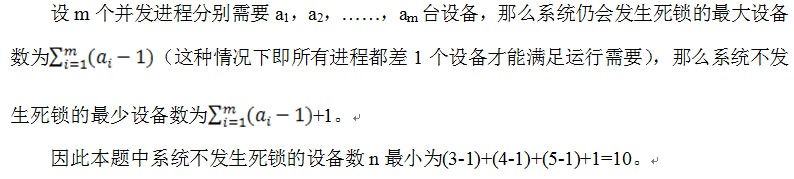
\includegraphics[width=8.27083in,height=1.86458in]{computerassets/596fce0cf07071e48e89e6d36a9a6089.jpeg}
\end{solution}
